\section{Superconducting Toroidal Magnet}\label{sec:clas.tor}

The essence of \abbr{CLAS} is the use of a toroidal magnetic field generated by six superconducting coils consisting of 4 layers of 54 windings of aluminum-stabilized niobium titanium NbTi/Cu superconductor \cite{clas}. The coils are separated in the azimuthal direction, $\phi$, by 60$^\circ$ and are located between Region-1 and Region-3 of the \abbr{DC}, see Fig~\ref{fig:clas.dc.torus.mag}. The placement of the coils is such that the magnetic field is encompassed by the volume of the \abbr{DC}, see Fig.~\ref{fig:clas.dc.torus.mag}. The direction of the toroidal field points along $\phi$, except near the coils,  such that the charged particles conserve their azimuthal angle along their trajectory, see Fig~\ref{fig:clas.dc.torus.cont}. The maximum current the magnet can support is 3861~A, resulting in a maximum field strength of 35~kG. During the \g12 experiment, the magnets operated at a current of 1930~A corresponding to a maximum field of about 20~kG. The field was oriented such that positive charged particles bent away from the beam-line, while negative charged particles bent toward the beam-line. Running at higher currents provides better momentum resolution but decreases the detector's acceptance for negative particles. Knowing the strength and direction of the magnetic field and the trajectory of a particle using the \abbr{DC}, the particle momentum can be determined by use of Eq.~\ref{eq:motioninmag}.
% During the \g12 experiment, the magnet was cooled down to 4.5~K using liquid helium ($\ell$He) obtained from the central CEBAF central cryogenic facility.

\begin{figure}[h!]\begin{center}
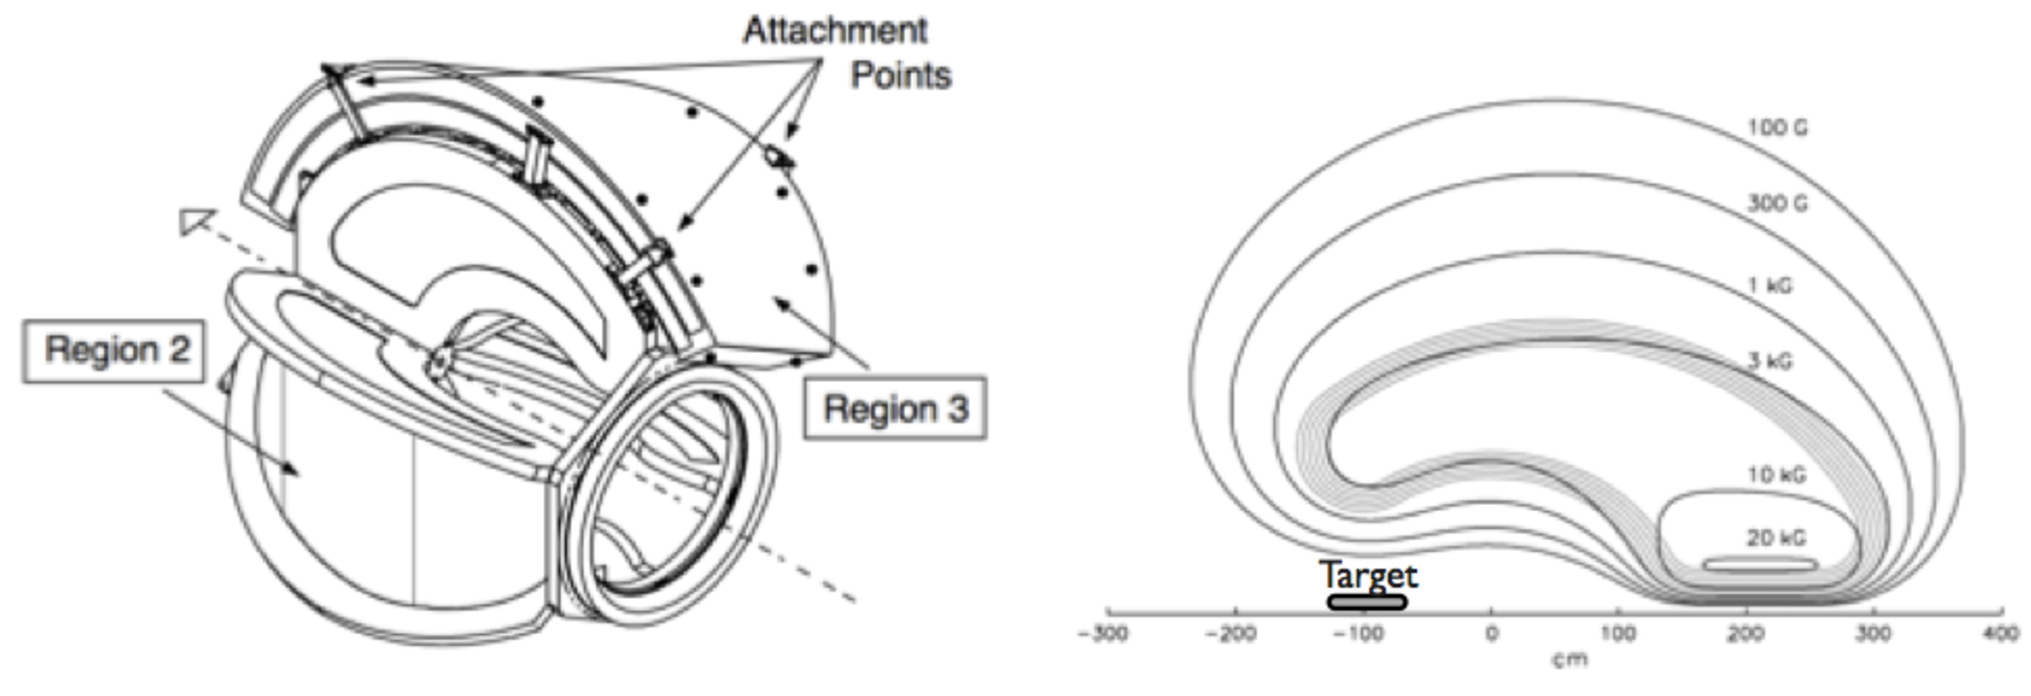
\includegraphics[width=\figwidth,height=0.9\qfigheight]{\figures/hall-b/torus_field_mag_mount.pdf}
\caption[The \abbr{CLAS} Superconducting Toroidal Magnet and its placement in relation to Region-1 and Region-3]{\label{fig:clas.dc.torus.mag}The \abbr{CLAS} Superconducting Toroidal Magnet and its placement in relation to Region-1 and Region-3  (left). Cross-section of the \abbr{CLAS} Superconducting Toroidal Magnet at half current (1930~A). Region-2 of the \abbr{DC} is located inside the region of the coils shown as the kidney shaped loop at about 3~kG (right).}
\end{center}\end{figure}

\begin{figure}[h!]\begin{center}
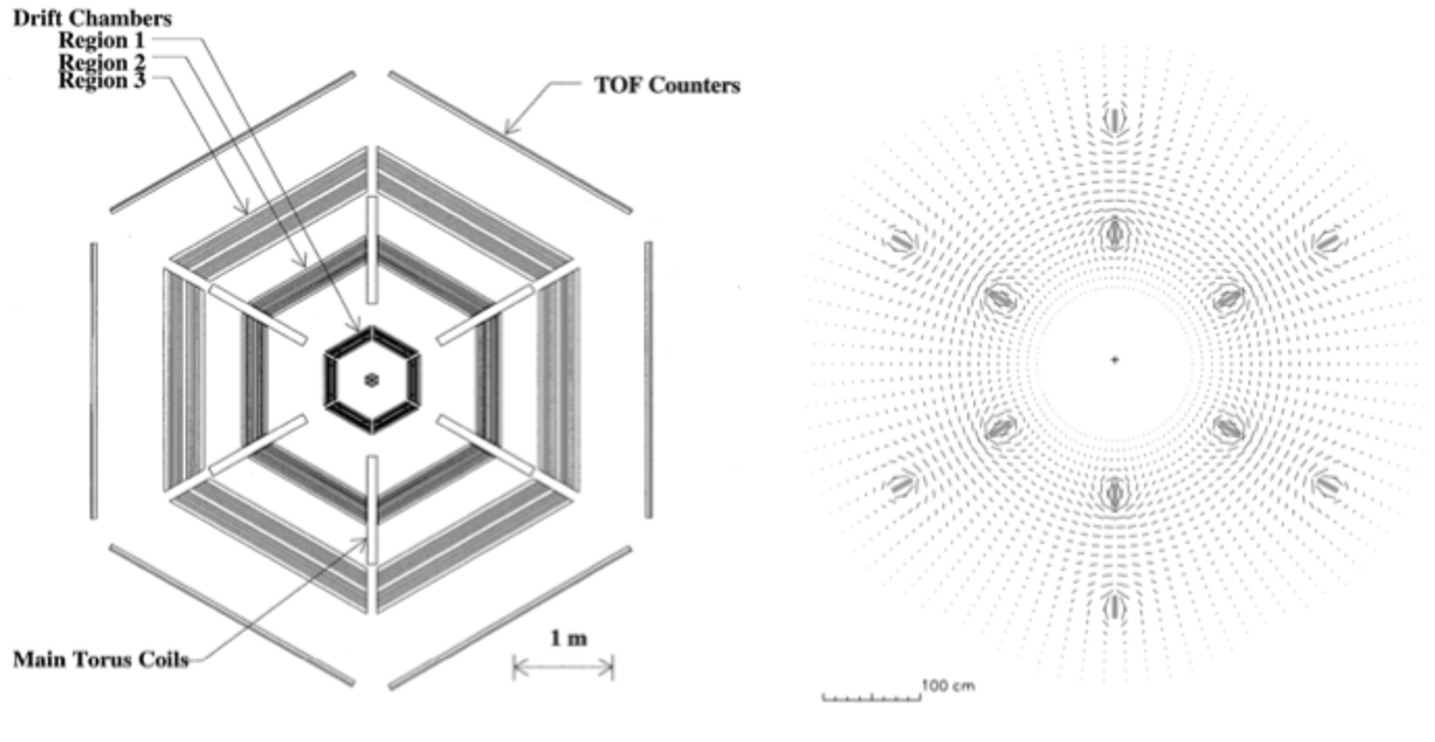
\includegraphics[width=1.\figwidth,height=0.75\hfigheight]{\figures/hall-b/torus_field_and_DC.pdf}
\caption[Schematic cross-sectional view of the \abbr{CLAS} detector, perpendicular to the beam line]{\label{fig:clas.dc.torus.cont}Schematic cross-sectional view of the \abbr{CLAS} detector, perpendicular to the beam line (left). The magnetic field distribution corresponding to the view in the left figure. The field is purely azimuthal. The six torus coils are shown in grey, the field is in the counter-clockwise direction,  the field strength is concentrated in the region between the coils (right).}
\end{center}\end{figure}

\FloatBarrier